\documentclass[]{article}
\usepackage{amsmath}
\usepackage{amssymb}
\usepackage{fullpage}
\usepackage{biblatex}
\usepackage{graphicx}
\usepackage{float}
\usepackage[hidelinks]{hyperref}
%opening 
\title{Bessel Functions: A Brief Introduction}
\author{Jonathan Haydak}

\begin{document}

\maketitle
\tableofcontents
\newcommand{\der}[1]{\frac{\partial}{\partial {#1}}}
\part{Bessel Functions}

\section{The Equation}
\begin{flushleft}
Now we will delve into some of the math behind Bessel Functions. We will begin at the natural starting place; Bessel's equation:
\begin{equation} \label{eq:beqn}
 x^2\frac{dy^2}{dx^2} + x \frac{dy}{dx} + (x^2-m^2)y = 0, \qquad m \in \mathbb{Z} 
\end{equation}
\eqref{eq:beqn} is traditionally referred to as Bessel's equation of order $m$. Being that this is a second order linear differential equation, it admits two linearly independent solutions. We will examine what is usually considered the fist sort of solution.
\end{flushleft}
\section{The First Solution: Bessel Functions of the First Kind}
\subsection{The solution form}
We will now attempt to solve \eqref{eq:beqn} and find a solution. To do so, we proceed by the method of Frobenius. Accordlingly, we assume a solution of the following form exists
\begin{equation} \label{eq:s1}
y(x) = x^r \sum_{n = 0}^{\infty} a_nx^n, \qquad r \in \mathbb{R}
\end{equation}
\subsection{Computing the solution where n is an integer}

Substituting \eqref{eq:s1} into \eqref{eq:beqn} yields
\begin{align*}
	0 &= x^2 \frac{d}{dx^2} \left( \sum_{n = 0}^{\infty} a_nx^{n+r} \right)+ x \frac{d}{dx} \left( \sum_{n = 0}^{\infty} a_nx^{n+r} \right)+ (x^2 - m^2)  \sum_{n = 0}^{\infty} a_nx^{n+r} \\
	&= x^2\left(\sum_{n=0}^{\infty}(n+r)(n+r-1)a_nx^{n+r-2} \right) + x \left(\sum_{n=0}^{\infty}(n+r)a_n x^{n+r-1}  \right) +  (x^2 - m^2)  \sum_{n = 0}^{\infty} a_nx^{n+r} \\
	&= \sum_{n=0}^{\infty}(n+r)(n+r-1)a_n x^{n+r} + \sum_{n=0}^{\infty}(n+r)a_nx^{n+r} +  \sum_{n = 0}^{\infty} a_nx^{n+r+2} - m^2 \sum_{n = 0}^{\infty} a_nx^{n+r} \\
	&= \sum_{n=0}^{\infty}(n+r)(n+r-1)a_n x^{n+r} + \sum_{n=0}^{\infty}(n+r)a_nx^{n+r} +  \sum_{n = 2}^{\infty} a_{n-2}x^{n+r} - m^2 \sum_{n = 0}^{\infty} a_nx^{n+r}
	\end{align*}
Now, since this sum must equal to 0, it follows that the coefficients for each power of x must also equal 0. Pulling out the  $x^r$ term of each sum we see that
\begin{align*}
	0 &= a_0x^r(r(r-1)+r-m^2) \\
	&= a_0x^r(r^2-m^2)
\end{align*}
Since $a_0 = 0$ will yield the trival solution, we must have that $r = \pm m$.  We will consider the case that $r = m$. 
\begin{align*}
	 0 &= \sum_{n=0}^{\infty}(n+m)(n+m-1)a_n x^{n+m} + \sum_{n=0}^{\infty}(n+m)a_nx^{n+m} +  \sum_{n = 2}^{\infty} a_{n-2}x^{n+m} - m^2 \sum_{n = 0}^{\infty} a_nx^{n+m}\\
	 & = ((m)(m-1)+m-m^2 )a_0x^m + \left((m+1)(m)+(m+1)-m^2\right)a_1x^{m+1} \\ 
	 &\qquad \qquad +\sum_{n=2}^{\infty}\left(\left((n+m)(n+m-1)+(n+m)-m^2\right)a_n + a_{n-2}\right)x^{n+m}
\end{align*}
As before, each coefficient must die for the expression to equal zero.
\begin{align}
		0 &=a_0x^m(m(m-1)+m-m^2) \nonumber \\
		& = 0 \nonumber \\
		&\implies a_0 \text{ is arbitrary} \nonumber \\
		0 & =a_1x^{m+1}((m+1)(m)+(m+1)-m^2 )\nonumber \\
		&= a_1(2m+1)x^{m+1} \nonumber \\
		& \implies a_1 = 0 \nonumber \\
		0 &= x^{m+2}\left((n+m)(n+m-1)+(n+m)-m^2\right)a_n + a_{n-2}) \nonumber \\
		&=n(n+2m)a_{n} + a_{n-2} \nonumber \\
		&\implies a_{n}=\frac{-a_{n-2}}{n(n+2m)} \label{eqn:cn1}
\end{align}
\subsection{Simplifying the solution}
Furthermore, with a little bit of algebraic manipulation it can be shown from \eqref{eqn:cn1} that
\begin{align}
	a_{2n} &= \frac{-a_{2n-2}}{2n(2n+2m)}, \qquad n > 0 \nonumber \\
	&=\frac{a_0(-1)^n}{2^{2n}n!(m+1)(m+2)+\ldots+(m+n)} \label{eqn:cn2}
\end{align}
Now, we make use of the gamma function, defined as follows where $z \in \mathbb{C}$ 
\[\Gamma(Z) = \int_{0}^{\infty}x^{z-1}\exp(-x)dx \]
Although this looks intimidating if you have not seen the gamma function before, the take home point is that for positive integers $n$, the gamma function has the property that $\Gamma(n) = (n-1)!$ which gives the useful identity $\Gamma(n+b+1)/\Gamma(n+1) = (n+1)(n+2)\ldots(n+b)$. Thus, \eqref{eqn:cn2} reduces to
\begin{equation}\label{eqn:cn3}
a_{2n} = \frac{(-1)^n\Gamma(m+1)a_0}{2^{2n}n!\Gamma(m+1+n)}
\end{equation}
Combining \eqref{eq:s1} and \eqref{eqn:cn3} we see that the solution is of the form
\begin{equation}
\sum_{n=0}^{\infty} \frac{(-1)^n\Gamma(m+1)a_0}{2^{2n}n!\Gamma(m+1+n)}
x^{2n+m}
\end{equation}
Now, it is customary to set $a_0$, which is arbitrary, to $a_0 = \frac{1}{\Gamma(m+1)2^m}$. Upon doing this, we get
 \begin{equation} \label{eqn:7}
 y(x) =\sum_{n = 0}^{\infty} \frac{(-1)^n}{n!\Gamma(m+n+1)}
 \left(\frac{x}{2}\right)^{2n+m}
 \end{equation}
 or, in a more reassuring form, which is true for the case that $m$ is an integer
 \begin{equation} \label{eqn:8}
 y(x) = \sum_{n=0}^{\infty}\frac{(-1)^n}{n!(m+n)!}
 \left(\frac{x}{2}\right)^{2n+m}
 \end{equation}
 
 By definition, \eqref{eqn:7} is called the \textbf{Bessel function of the first kind of order m} and is denoted $J_m(x)$.
 \section{Non-integer solutions}
 You might have noticed that the introduction of the gamma function was rather superfluous. You would be correct; in the case of integers we can get away with just using factorials, but \eqref{eqn:7} is true \textit{even when }$m$\textit{ is not an integer.}
 
 However, there are some special cases, most notably the cases where $m$ is a half integer. We will example the simplest case. Suppose $m = \pm \frac{1}{2}$. We will retain our choice of $a_0$. In this case, we can write a closed form solution of $J_{\frac{1}{2}}(x)$ and $J_{-\frac{1}{2}}(x)$; we will show the former first.
 
 \subsection{Half integer case: $m$ = 1/2}
  Accordingly, we return to \eqref{eqn:cn1} to re-calculate the coefficients. We saw that in the integer case, 
 \[a_n = \frac{-a_{n-2}}{n(n+2m)}\]
 so now
 \begin{equation} \label{eq:9}
 	a_n = \frac{-a_{n-2}}{n(n+1)}
 \end{equation}
 and it follows for $n > 0$
 \begin{align*}
 	a_{2n} &= \frac{-a_{2n-2}}{2n(2n+1)} \\
 		&= \frac{(-1)^na_0}{2^nn!
 		(3)(5)(7)\ldots(1+2n)}\\
 \end{align*}
 Observe that 
 \[
 1  \times 3 \times 5 \times \ldots \times (1+2n) = \frac{(1+2n)!}{2^n(n!)}
 \]
 From which we see
 \begin{align}
 		a_{2n} &= \frac{(-1)^na_0}{(1+2n)!}
 \end{align}
 Using the same choice of $a_0$ as before, we get that $a_0 = \frac{1}{\Gamma(\frac{3}{2})2^{\frac{1}{2}}}$.
 \begin{align*}
	 \Gamma(\frac{3}{2}) &= \int_{0}^{\infty}\sqrt{x}\exp(-x)dx\\
	 & = \frac{1}{2}\sqrt{\pi}
 \end{align*}
 With the previous integral being calculated by all sorts of horrible black magic I do not wish to get into. It follows that
 \[a_0 = \frac{2}{\sqrt{\pi}\sqrt{2}} = \sqrt{\frac{2}{\pi}} \]
Thus, if we factor out an $x^{-.5}$ term, we get 
\begin{align} 
	J_{\frac{1}{2}}(x) &=x^{-.5} \sqrt{\frac{2}{\pi}} \sum_{n=0}^{\infty}
	\frac{(-1)^n}{(1+2n)!}
	x^{2n+1}\\
	&\frame{$\displaystyle =	\sqrt{\frac{2}{x\pi}}\sin(x)$}
 \end{align}
\subsection{Half integer case: m = -1/2}
This process is very similar to the previous. In this case, going back to \eqref{eqn:cn3}, we see that 
\begin{equation}
	a_n = \frac{-a_{n-2}}{n(n-1)}
\end{equation}
and we follow the same procedure as before.
\begin{align}
	a_{2n} &= \frac{-a_{2n-2}}{2n(2n-1)}, \qquad n > 0\\
	&= \frac{(-1)^na_0}{2^nn!(1)(3)(5)(2n-1)} \nonumber \\
	&=\frac{(n-1)!2^{n-1}(-1)^na_0}{2^nn!((2n-1)!} \nonumber \\
	& = \frac{(-1)^na_0}{(2n)!}
\end{align}
For the computation of $a_0$, we will refer to a table of integrals and defer computing the actual integral.
\begin{align*}
	a_0 & = \frac{1}{\Gamma(1/2) 2^{-.5}}\\
		&=  \frac{\sqrt{2}}{\sqrt{\pi}}\\
		&= \sqrt{\frac{2}{\pi}}
\end{align*}
Finally, plugging in $a_n$
\begin{align}
	J_{-\frac{1}{2}}(x) &=  \sqrt{\frac{2}{\pi}} \sum_{n = 0}^{\infty}
	\frac{(-1)^n}{(2n)!} 
	x^{2n-.5} \nonumber \\
	&=  \sqrt{\frac{2}{x\pi}} \sum_{n = 0}^{\infty}
	\frac{(-1)^n}{(2n)!}
	x^{2n} \\
	&\frame{$\displaystyle =\sqrt{\frac{2}{x\pi}} \cos(x)$}
\end{align}
\subsection{Comments on Closed Form Solutions}
It is possible to find closed form solutions of other special values of $m$, but most of them are some variant of a decaying sine or cosine signal.

\section{Second Solution to Bessel's Equation}
\subsection{Two Solutions of the first kind}
As stated earlier, \eqref{eq:beqn} should have two linearly independent solutions by virtue of being second order. If you are familiar with the method of Frobenius, your first instinct might be to try the $-m$ root obtained from the indicial equation.

Sometimes this works. Sometimes it doesn't. To be more precise, $J_{-m}(x)$ is a second linearly independent solution only when $m$ is \textbf{not} an integer. We will go through why it fails - but won't prove that it doesn't for non-integers, as that involves shenanigans with gamma functions.

Suppose $m$ is an integer. Then,

\begin{align*}
	J_{m}(x) &=\sum_{n = 0}^{\infty} \frac{(-1)^n}{n!\Gamma(m+n+1)}
	 \left(\frac{x}{2}\right)^{2n+m}\\
 	&= \sum_{n=0}^{\infty}\frac{(-1)^n}{n!(m+n)!}
	 \left(\frac{x}{2}\right)^{2n+m} \\
\end{align*}

Where we stress the second equivalence is only for integers. Now, the gamma function and therefore factorials are not defined for numbers with negative real parts. Thus, we must shift the index to account for this when giving the solution form of $J_{-m}$.
\begin{align}
 J_{-m}(x) &=\sum_{n-m+1 > 0}^{\infty} \frac{(-1)^n}{n!\Gamma(-m+n+1)}
 	 \left(\frac{x}{2}\right)^{2n-m} \label{eq:njm}\\
 	 &=\sum_{n-m \geq 0}^{\infty}\frac{(-1)^n}{n!(-m+n)!}
 	\left(\frac{x}{2}\right)^{2n-m} \label{eq:njm2}
\end{align}

Changing the index from $n \to n-m$

\begin{align}
 J_{-m}(x) &=\sum_{n=0}^{\infty}\frac{(-1)^{n+m}}{(n+m)!(n)!}
 	\left(\frac{x}{2}\right)^{2n+m} \label{eq:njm4}\\
 	&= (-1)^m J_{m}(x) \label{eq:intid}
\end{align}

By \eqref{eq:intid}, we cannot have two linearly independent solutions of the first kind, and so we must take drastic measures to construct a second solution.
\newpage
\subsection{Bessel Functions of the Second Kind}
Consider the function
\begin{equation} \label{eq:2nd}
Y_m(x) = \frac{J_m(x)\cos(m\pi)-J_{-m}(x)}{\sin(m\pi)}
\end{equation}
Since \eqref{eq:2nd} is not well defined for integer orders, the convention is to take $Y_n(x) = \lim\limits_{a \to n} Y_{a}(x)$ where $n$ is an integer.

$Y_m(x)$ is called a Bessel Function of the Second Kind of order $m$. This class of functions is also called the Neumann functions. Let's take a second to look at what this is. For $m$ not an integer, $Y_m(x)$ just a linear combination of $J_m(x)$ and $J_{-m}(x)$ and so it is also a solution to Bessel's Equation.

\subsection{Preliminary Work and a Few Identities}
Before we can examine the Neumann functions, we have to present a few ideas and concepts that we just cannot avoid. Brace yourself.
\subsubsection*{Abel's Identity}
From Abel's identity, given an equation of the form $ \frac{d^2y}{{dx}^2} + p \frac{dy}{dx} + qy = 0$,
{\Large
\begin{equation}
	 W[y_1,y_2] (x) = Ce^{-\int_{x_0}^{x}p(t)dt)}
\end{equation}}

\subsubsection*{Derivative of $J_m(x)$: Integer case}
We begin with the series form of $J_m(x)$. We will also assume that $m > 0$ and note that $m=0$ is a rather simple case. 
\begin{align*}
	J'_m(x) & = \frac{d}{dx}\sum_{n=0}^{\infty}\frac{(-1)^n}{n!(m+n)!}
		 \left(\frac{x}{2}\right)^{2n+m} \\
	&= \sum_{n=0}^{\infty}\frac{(-1)^n}{n!(m+n)!}
	\frac{d}{dx}\left(\frac{x}{2}\right)^{2n+m} \\
	&=\frac{1}{2}\sum_{n=0}^{\infty}\frac{(2n+m)(-1)^n}{(n!)(m+n)!}
	\left(\frac{x}{2}\right)^{2n+m-1} \\
	&= \frac{1}{2}\sum_{n=0}^{\infty}\frac{2n(-1)^n}{(n!)(m+n)!}
	\left(\frac{x}{2}\right)^{2n+m-1} +
	\frac{1}{2}\sum_{n=0}^{\infty}\frac{m(-1)^n}{(n!)(m+n)!}
	\left(\frac{x}{2}\right)^{2n+m-1} \\
	&= \sum_{n=0}^{\infty}\frac{(-1)^n}{(n-1)!(m+n)!}
	\left(\frac{x}{2}\right)^{2n+m-1} +
	\frac{m}{2}\sum_{n=0}^{\infty}\frac{(-1)^n}{(n!)(m+n)!}
	\left(\frac{x}{2}\right)^{2n+m-1} \\
	\intertext{Change the index $n \to n+1$ on the left sum and factor out $\left(\frac{x}{2}\right)^{-1}$ from the right sum}\\
	&= \sum_{n = 0}^{\infty}\frac{(-1)^{n+1}}{(n)!(n+m+1)!}
	\left(\frac{x}{2}\right)^{2n+m+1} +
	\frac{m}{x}\sum_{n=0}^{\infty}\frac{(-1)^n}{(n!)(m+n)!}
	\left(\frac{x}{2}\right)^{2n+m} \\
\end{align*}
And finally, expressing this using conventional notation, 
\begin{equation} \label{derivid1}
	\boxed{J'_m(x) = -J_{m+1}(x) + \frac{m}{x} J_m(x) }
\end{equation}
Now, recall \eqref{eq:intid} where we showed that for integers $J_{-m}(x) = (-1)^mJ_m(x)$. Combining this result with \eqref{derivid1}, we see that
\begin{align}
	J'_{-m}(x) &= -J_{-m+1}(x) - \frac{m}{x} J_{-m}(x) \nonumber \\
	(-1)^mJ_{m}(x) &= -(-1)^{-m+1}J_{m-1}(x) -\frac{m}{x} (-1)^m J_m(x) \nonumber 
\end{align}
\begin{equation}	\label{derivid2}
	\boxed{ J'_{m}(x) = J_{m-1}(x) -\frac{m}{x} J_m(x)   }
\end{equation}
Upon adding \eqref{derivid1} and \eqref{derivid2}, we come up with the following relation.
\begin{equation} \label{derivid3}
	\boxed{
	J'm(x) = \frac{1}{2}\left[J_{m-1}(x) - J_{m+1}(x) \right]
	}
\end{equation}
\subsection{A deeper look at $Y_m(x)$ for integer cases}
For integer cases, we defined $Y_m(x)$ in the following manner.
\begin{align*}
	Y_m(x) &= \lim\limits_{v \to m} \frac{J_v(x)\cos(\pi v) - J_{-v}(x)}{\sin(\pi v)}\\
	\intertext{Which for integers yields an indeterminate form. Thus, applying L'Hospital's rule:} \\
	&= \lim\limits_{v \to m} \frac{\frac{\partial \, J_v(x)}{\partial v}\cos(\pi v) - \pi J_v(x)\sin(\pi v) -\frac{\partial}{\partial v}J_{-v}(x)}{\pi \cos(\pi v)}\\
	&=-\lim\limits_{v \to m}\frac{1}{\pi (-1)^m} \left[ 
	(-1)^m\frac{\partial \, J_v(x)}{\partial v} - 
	\frac{\partial \, )J_{-v}(x)}{dv}
	\right] \\
\end{align*}
Which reduces to
\begin{equation} \label{eq:yn1}
	Y_m(x)=\lim\limits_{v \to m} \frac{1}{\pi}\left[ \frac{\partial\, J_v(x)}{\partial v} - (-1)^m \frac{\partial \, J_{-v}(x)}{\partial v}\right]
\end{equation}		

To further simplify this, we need to find a suitable equivalent form of $\frac{\partial}{\partial v} J_v(x) $.

\begin{align*}
	\frac{\partial}{\partial v} J_v(x) &= \frac{\partial}{\partial v} \sum_{n = 0}^{\infty} \frac{(-1)^n}{n!\Gamma(v+n+1)}
		 \left(\frac{x}{2}\right)^{2n+v}\\
\end{align*}
Here we note that
\begin{align*}
 	\der{v}\left[\left(\frac{x}{2}\right)^{2n+v}\right] &= \der{v} e^{(2n+v)\ln(\frac{x}{2})}\\
 	&= e^{2n\ln(\frac{x}{2})} \der{v} e^{v\ln(\frac{x}{2})} \\
 	&= e^{2n\ln(\frac{x}{2})}  e^{v\ln(\frac{x}{2})} \ln(\frac{x}{2}) \\
 	&= \left(\frac{x}{2}\right)^{2n+v}\ln(\frac{x}{2})
\end{align*}
And also
\begin{align*}
	\der{v}\left( \frac{1}{\Gamma(1+v+n)}\right) &= - \frac{1}{\left(\Gamma(1+v+n)\right)^2} \left(\Gamma(1+v+n)\Psi _0(1+v+n)\right)\\
	&= -\frac{\Psi _0(1+v+n)}{\Gamma(1+v+n)}
\end{align*}
Where $\Psi$ is the digamma function, another magical and mystic mathematical artifact which we will not delve into.
Now, returning to the earlier expression:
\begin{align*}
	\frac{\partial}{\partial v} J_v(x) &= \frac{\partial}{\partial v} \sum_{n = 0}^{\infty} \frac{(-1)^n}{n!\Gamma(v+n+1)}
		\left(\frac{x}{2}\right)^{2n+v}\\
		 &= \sum_{n=0}^{\infty}\left[ \frac{(-1)^n -\Psi _0(1+v+n)}{n!\Gamma(1+v+n)} \left(\frac{x}{2}\right)^{2n+v}
		 +\left(\frac{x}{2}\right)^{2n+v}\ln(\frac{x}{2})
		  \frac{(-1)^n}{n!\Gamma(v+n+1)}
		 \right] \\
		 &= \sum_{n=0}^{\infty}  \frac{(-1)^n}{n!\Gamma(v+n+1)}	\left(\frac{x}{2}\right)^{2n+v} \left(
		 -\Psi _0(1+v+n) + \ln(\frac{x}{2})
		 \right) \\
		 &= \ln(\frac{x}{2}) J_v(x) - \sum_{n=0}^{\infty} \frac{(-1)^n \Psi _0(1+v+n)}{n!\Gamma(1+v+n)}	\left(\frac{x}{2}\right)^{2n+v}\\
		 \intertext{Now we make use of the identity that holds for positive integer values of $x$: $\Psi_0(n+1) = - \gamma + \sum\limits_{k = 1}^{n} \frac{1}{k}$ where $\gamma$ is Euler's constant.}\\
		 &=  \ln(\frac{x}{2}) J_m(x) - \sum_{n=0}^{\infty} \frac{(-1)^n }{n!\Gamma(1+v+n)}	\left(\frac{x}{2}\right)^{2n+v}
		 \left(- \gamma + \sum_{k = 1}^{v+n} \frac{1}{k}
		 \right)
\end{align*}	
\begin{equation} \label{eq:pderiv1}
\boxed{
		 =  \left( \ln(\frac{x}{2}) - \gamma \right) J_v(x) - \sum_{n=0}^{\infty} \frac{(-1)^n(1 + \frac{1}{2} + \ldots + \frac{1}{v+n}) }{n!\Gamma(1+v+n)} 	\left(\frac{x}{2}\right)^{2n+v}
		 }
\end{equation}		

Although similar, it is often convenient to split the corresponding expression for $J_{-v}(x)$ into two sums because now we have to conside negative arguments of the gamma function:
\begin{align*}
	\der{v} J_{-v}(x) &= \der{v} \left[ \sum_{n = 0}^{m-1} 	\frac{(-1)^n}{n!\Gamma(-v+n+1)} + \sum_{n = m}^{\infty} 	\frac{(-1)^n}{n!\Gamma(-v+n+1)}\right]
 	 \left(\frac{x}{2}\right)^{2n-v}\\
 	 \intertext{Now we use the following identity}
\end{align*}
\begin{align*}
 	  \frac{1}{\Gamma(1-v+n)\Gamma(1+v-n)} &= \frac{\sin(\pi(v-n))}{\pi(v-n)} \\
 	  \implies \frac{1}{\Gamma(1-v+n)} &= \frac{\Gamma(1+v-n)\sin(\pi(v-n))}{\pi(v-n)} \\
 	  &= \frac{\Gamma(v-n)\sin(\pi(v-n))}{\pi}
 	  \intertext{And now we calculate the derivative with respect to $v$:}\\
 	  \der{v}\left(\frac{1}{\Gamma(1+v-n)}\right) &= \frac{1}{\pi} \left( \Gamma(v-n)\Psi_0(v-n)\sin(\pi(v-n)) + \pi\Gamma(v-n)\cos(\pi(v-n)) \right)
\end{align*}
Hence,
\begin{equation} \label{eq:jnegvid}
\boxed{
		\der{v} J_{-v}(x) = \sum_{n=0}^{m-1} \frac{\Gamma(v-n)(-1)^{v} \left(
		\frac{x}{2}\right)^{2n-v}}{n!}
		+ \sum_{n=v}^{\infty} \frac{(-1)^n\Psi_0(n-v+1)}{n!\Gamma(n-v+1)} \left(\frac{x}{2}\right)^{2n-v}
		- \sum_{n = m}^{\infty} \frac{(-1) ^n}{n!\Gamma(n-v+1)}\ln\left( \frac{x}{2} \right) \left( \frac{x}{2} \right) ^{2n-v} }
\end{equation}
\subsubsection*{Series form of $Y_n(x)$ for integral orders}
Combining the previous slew of results with \eqref{eq:yn1}, we see the following:
\begin{align}
	Y_m(x)&=\lim\limits_{v \to m} \frac{1}{\pi}\left[ \frac{\partial\, J_v(x)}{\partial v} - (-1)^m \frac{\partial \, J_{-v}(x)}{\partial v}\right] \nonumber \\
	&= \lim\limits_{v \to m}\frac{1}{\pi} \Bigg[
	\left( \ln(\frac{x}{2}) - \gamma \right) J_v(x) - \sum_{n=0}^{\infty} \frac{(-1)^n(1 + \frac{1}{2} + \ldots + \frac{1}{v+n}) }{n!\Gamma(1+v+n)} 	\left(\frac{x}{2}\right)^{2n+v} 
	- (-1)^m \sum_{n=0}^{m-1} \frac{\Gamma(v-n)(-1)^{v} \left(
	\frac{x}{2}\right)^{2n-v}}{n!} \nonumber \\
	& \qquad - (-1)^m \sum_{n=v}^{\infty} \frac{(-1)^n\Psi_0(n-v+1)}{n!\Gamma(n-v+1)} \left(\frac{x}{2}\right)^{2n-v}
	+ (-1)^m \sum_{n = m}^{\infty} \frac{(-1) ^n}{n!\Gamma(n-v+1)}\ln\left( \frac{x}{2} \right) \left( \frac{x}{2} \right) ^{2n-v} \Bigg] 
\end{align}
Now we use the identity for $\Psi_0$ used in \eqref{eq:pderiv1} and take the limit as $v \to m$
\begin{align}
	Y_m(x)&= \frac{1}{\pi}\left( \ln(\frac{x}{2}) - \gamma \right) J_m(x) - \frac{1}{\pi}\sum_{n=0}^{\infty} \frac{(-1)^n(1 + \frac{1}{2} + \ldots + \frac{1}{m+n}) }{n!\Gamma(1+m+n)} 	\left(\frac{x}{2}\right)^{2n+m} 
	- \frac{1}{\pi} \sum_{n=0}^{m-1} \frac{\Gamma(m-n) \left(\frac{x}{2}\right)^{2n-m}}{n!} \nonumber \\
	& \qquad - \frac{(-1)^m}{\pi} \sum_{n=m}^{\infty} \frac{(-1)^n(-\gamma + (1 + \frac{1}{2} + \ldots + \frac{1}{n-m})  )}{n!\Gamma(n-m+1)} \left(\frac{x}{2}\right)^{2n-m} + \frac{(-1)^m}{\pi} \sum_{n = m}^{\infty} \frac{(-1) ^n}{n!\Gamma(n-m+1)}\ln\left( \frac{x}{2} \right) \left( \frac{x}{2} \right) ^{2n-m}
\end{align}
We factor out the $\ln$ term in the last sum and convert it to the proper $J_m(x)$ function. We also do the same with the $\gamma$ in the second to last sum.
\begin{align}
	Y_m(x)&= \frac{2}{\pi}\left( \ln(\frac{x}{2}) - \gamma \right) J_m(x) - \frac{1}{\pi}\sum_{n=0}^{\infty} \frac{(-1)^n(1 + \frac{1}{2} + \ldots + \frac{1}{m+n}) }{n!\Gamma(1+m+n)} 	\left(\frac{x}{2}\right)^{2n+m} 
	- \frac{1}{\pi} \sum_{n=0}^{m-1} \frac{\Gamma(m-n) \left(\frac{x}{2}\right)^{2n-m}}{n!} \nonumber \\
	& \qquad - \frac{(-1)^m}{\pi} \sum_{n=m}^{\infty} \frac{(-1)^n(1 + \frac{1}{2} + \ldots + \frac{1}{n-m})  }{n!\Gamma(n-m+1)} \left(\frac{x}{2}\right)^{2n-m} 
\end{align}
Shift the index of the last two sums by $m$ and substitute in the appropriate factorials
\begin{align}
	Y_m(x)&= \frac{2}{\pi}\left( \ln(\frac{x}{2}) - \gamma \right) J_m(x) - \frac{1}{\pi}\sum_{n=0}^{\infty} \frac{(-1)^n(1 + \frac{1}{2} + \ldots + \frac{1}{m+n}) }{n!(m+n!)} 	\left(\frac{x}{2}\right)^{2n+m} 
	- \frac{1}{\pi} \sum_{n=0}^{m-1} \frac{(m-n-1)! \left(\frac{x}{2}\right)^{2n-m}}{n!} \nonumber \\
	& \qquad - \frac{(-1)^m}{\pi} \sum_{n=0}^{\infty} \frac{(-1)^{n+m}(1 + \frac{1}{2} + \ldots + \frac{1}{n})  }{(n+m)!n!} \left(\frac{x}{2}\right)^{2n+m} 
\end{align}
Combining like terms, we come to a series expression of $Y_m(x)$ for integer cases.
\begin{equation} \label{eq:Yseries}
	\boxed{
	\begin{aligned}
	Y_m(x)&= \frac{2}{\pi}\left( \ln(\frac{x}{2}) - \gamma \right) J_m(x) 
	- \frac{1}{\pi} \sum_{n=0}^{m-1} \frac{(m-n-1)! \left(\frac{x}{2}\right)^{2n-m}}{n!}  \\
	& \qquad - \frac{1}{\pi} \sum_{n=0}^{\infty} \frac{(-1)^{n}  }{(n+m)!n!} ((1 + \frac{1}{2} + \ldots + \frac{1}{n}) + (1+ \frac{1}{2} + \ldots + \frac{1}{m+n})\left(\frac{x}{2}\right)^{2n+m}
	\end{aligned} 
	}
\end{equation}
Now, one thing to note is that there are other series forms of $Y_m(X)$, but the derivation of one is enough of a demonstration to show how involved a process it is.
\subsection*{(Outline of)Proof of Linear Independence of $Y_m(x)$}
Up until now, we have not provided a formal proof or argument that $Y_m(x)$ and $J_m(x)$ are linearly independent. Although from just looking at the definition of $Y_m(x)$, you might suspect that this is the case. In fact, for non-integer cases we merely have to observe that it is a linear combination of $J_m(x)$ and $J_{-m}(x)$ to see that it is linearly independent.

Expressing Bessel's equation in the appropriate form to use Abel's identity, we have that 
\begin{equation} \label{eqn:stdbessel}
	\frac{d^2y}{{dx}^2} + \frac{1}{x}\frac{dy}{dx} + (1 - \frac{m^2}{x^2})y = 0
\end{equation}
From Abel's identity, we have that
\begin{align}
	W[y_1,y_2] &= C e^{-\int_0^x \frac{1}{t}dt} \\
	&= Ce^{-\log(x)} \nonumber \\
	&= \frac{C}{x}
\end{align}
Or equivalently,
\begin{equation} \label{eq:abelidresult}
	y_1y_2' - y_1'y_2 = \frac{C}{x} 
\end{equation}
However, we already know that one solution to Bessel's equation is $J_m(x)$:
\begin{equation} \label{eq:abelr2}
	J_m(x)y' - yJ'_m(x) = \frac{C}{x}
\end{equation}
Since clearly $Y_m(x)$ is a solution to \eqref{eqn:stdbessel}, to prove linear independence it suffices to show that the $C$ value of $W[J_m(x),Y_m(x)]$ is nonzero. We may compute \eqref{eq:abelidresult} at any $x \in (0,\infty)$. We will not go through this derivation, but will instead suggest a clever way of proving this outlined in Watson's work on Bessel Functions. \footcite{Watson: A Treatise on the Theory of Bessel Functions, 2nd ed}

First, compute $W[J_m(x),J_{-m}(x)]$ for the general case. Observe that the result can be expressed in terms of the lowest power of $x$ appearing in the sum plus an error term, $O(x)$. The resulting lowest power of $x$ will be $\frac{1}{x}$. Combining this with \eqref{eq:abelidresult}, it follows that the resulting $O(x)$ must vanish, leaving a single term proportional to $\frac{1}{x}$. From this, the result for $Y_m(x)$ can be obtained, and it will be nonzero.
\subsection{Alternative way of computing series of $Y_m(x)$ for integer $m$)}
The following method is based on Abel's identity. Starting \eqref{eq:abelr2}, we see that
\begin{align}
	J_m(x)y' - yJ'_m(x) &= \frac{C}{x} \nonumber \\
	\intertext{dividing both sides by $J_m(x)^2$ gives} \nonumber\\
	\left(\frac{y}{J_m(x)}\right)' &= \frac{C}{x\left(J_m(x)\right)^2} \nonumber \\
	 y &= AJ_m(x)\int \frac{dx}{x\left(J_m(x) \right)^2} \label{eq:abelr3}
\end{align}
From here, all that remains is plugging in for the power series of $J_m(x)$ and then doing the appropriate calculations, which will result in a series form of a second linearly independent solution.

\section{Numerical Approximation and Plots}
\subsection{Basic Algorithm}
Many mathematical programming packages already have built in programs or support for bessel functions. Although these will suffice for most applications, let's very briefly see how to do it. The case for Bessel functions of the first type is very simple, for instance, given a value of x and an order, we may find $J_m(x)$ numerically in the following manner:
\begin{enumerate}
	\item Set $f$ = 0. Set numTerms as the number of terms in the power series to be computed.
	\item If $m >0$, set lowersum = 0. Otherwise, if $m$ is an integer, set lowersum = $-m$. If $m$ is not an integer, set lowersum = ceil($-1-m$). Set $n$ = lowersum.
	\item If n = numTerms, go to step 6. Otherwise, compute $a_{2n}$ using the formula \eqref{eqn:7}. Multiply this by $\frac{x}{2}^{2n+m}$ and add the value to $f$. 
	\item set $n = n + 1$.
	\item Repeat steps 3-5.
	\item Return $f$
\end{enumerate}
However, computing $Y_m(x)$ is a bit more tricky, but not impossible. The most straightforward way to do this is to use the series in \eqref{eq:Yseries} in its form with Gamma functions. However, the series is rather bulky and it seems a bit more natural to merely calculate $Y_m(x)$ from the definition. 

However, we have a problem once we try and tackle the case of integer orders. Any method that computes $J_m(x)$ based on a power series is going to return a series that is bounded at the origin - namely having a value of $0$ for $x = 0$ with the exception of $1$ for order 0 Bessel functions of the first kind. We solve this by calculating $J_{\pm(m-\epsilon)}(x)$ for some arbitrarily small value of $\epsilon$. 

The resulting series converges rather quickly; and the accuracy is very high. For most applications, computing Bessel functions in this matter should suffice. Another simple way of computing $Y_m(x)$ is using \eqref{eq:abelr3}.
\subsection{Plots}
\begin{figure}[H]
\centering
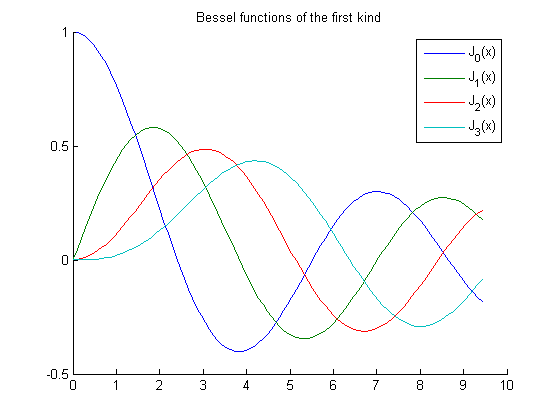
\includegraphics[width=0.7\linewidth]{./j1}
\caption{$J_m(x)$ for $ 0 \leq m \in \mathbb{Z} \leq 3$}
\label{fig:j1}
\end{figure}

\begin{figure}[H]
\centering
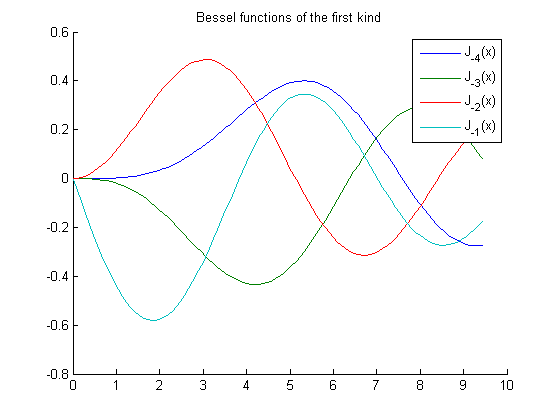
\includegraphics[width=0.7\linewidth]{./j2}
\caption{$J_m(x)$ for $ -4 \leq m \in \mathbb{Z} \leq -1$}
\label{fig:j2}
\end{figure}

\begin{figure}[H]
\centering
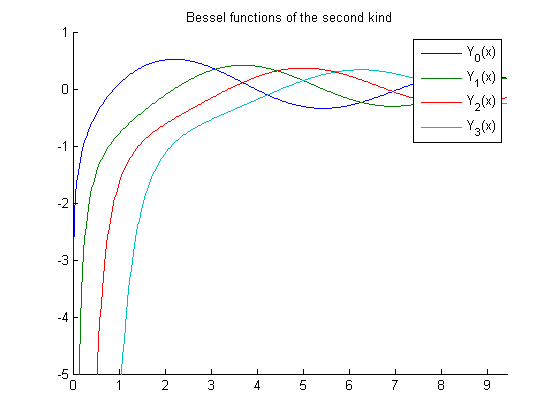
\includegraphics[width=0.7\linewidth]{./y3}
\caption{$Y_m(x)$ for $ 0 \leq m \in \mathbb{Z} \leq 3$}
\label{fig:y3}
\end{figure}

\begin{figure}[H]
\centering
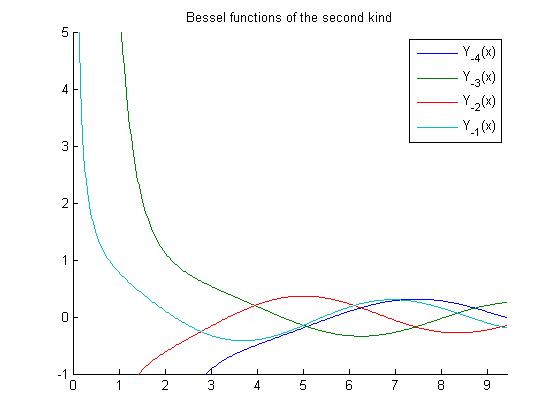
\includegraphics[width=0.7\linewidth]{./y4}
\caption{$Y_m(x)$ for $ -4 \leq m \in \mathbb{Z} \leq -1$}
\label{fig:y4}
\end{figure}



\part{Variations on the Bessel Functions/Equation}
By slightly altering Bessel's Equation, we change the solution set and the properties of the solutions slightly. Although different from the standard Bessel Functions and equation, the theory behind them is intertwined.
\section{Modified Bessel Functions}
Consider the slightly modified equation 
\begin{equation} \label{eq:modbes}
	x^2 \frac{d^2 \,y }{dx^2} + x \frac{d \, y}{dx} - (x^2 + n^2)y =0
\end{equation}
\eqref{eq:modbes} is called the Modified Bessel Equation. The only difference is that the $x$ in the last term has been substituted for $ix$. As before, we will seek out a fundamental set of solutions. Accordingly, we proceed by the method of frobenius and assume a solution of the form $y = x^r \sum\limits_{k = 0}^{\infty} a_k x^k$.
\begin{align*}
	0 &= \sum_{k=0}^{\infty}(k+r)(k+r-1)a_kx^{k+r} + \sum_{k=0}^{\infty}(k+r)a_kx^{k+r} - \sum_{k=0}^{\infty}a_kx^{k+r+2} - \sum_{k=0}^{\infty}n^2a_kx^{k+r}\\
	&= \sum_{k=0}^{\infty}(k+r)(k+r-1)a_kx^{k+r} + \sum_{k=0}^{\infty}(k+r)a_kx^{k+r} - \sum_{k=2}^{\infty}a_{k-2}x^{k+r} - \sum_{k=0}^{\infty}n^2a_kx^{k+r}\\
	&= \left((r)(r-1)+r-n^2 \right)a_0x^r
	+ \left((1+r)(r)+(r+1)-n^2 \right)a_1x^{1+r} \\
	&\qquad + \sum_{k=2}^{\infty}
	\left(
	\left((k+r)(k+r-1)+(k+r)-n^2\right)a_k - a_{k-2}
	\right) x^{k+r}\\
	&= (r^2-n^2)a_0x^r + (r^2+2r+1-n^2)a_1x^{1+r} + \sum_{k=2}^{\infty} \left(
	(k^2+2kr+r^2-n^2)a_k - a_{k-2}
	\right)x^{k+r}
\end{align*}
It follows that $r = \pm n$, and $a_1 = 0$. Moreover,  $\displaystyle a_k = \frac{a_{k-2}}{k^2+2kr+r^2-n^2}$. Consider $r = n$.

\begin{align*}
	a_k &= \frac{a_{k-2}}{k(k+2n)} \\
	\implies a_{2k} &= \frac{a_{2k-2}}{2k(2k+2n)} \\
	&= \frac{a_{0}\Gamma(k+n)}{2^{2k}k!\Gamma(k+n+1)}
\end{align*}
Taking the same value of $a_0$ as before, basically whatever value kills the $\Gamma$ on top and the excess 2, yields the solution
\begin{equation} \label{eq:msol1}
	y = I_n(x) = \sum_{k=0}^{\infty} \frac{1}{k!\Gamma(k+n+1)} \left(\frac{x}{2}\right)^{2k+n}
\end{equation}
\eqref{eq:msol1} is called a modified Bessel functions of the first kind and denoted $I_n(x)$. Something worthy of noting immediately is that 
\[
	i^{-n}J_n(ix) = \sum_{k=0}^{\infty}\frac{1}{k!\Gamma(k+n+1)}\left(\frac{x}{2}\right)^{2k+n} = I_n(x)
\]
\subsection*{Modified Bessel functions of the second kind}
As before, the second solution is defined in much the same way as it's analog to the unmodified situation. 

If $m$ is not an integer, then 
\begin{equation}
	K_m(x) = \frac{\pi}{2} \frac{I_{-m}-I_m(x)}{\sin(m\pi)}
\end{equation}
for integers, we take the limit as the order $\to m$.
\section{Parametric Bessel Equation and Fourier-Bessel Series}
\subsection{Parametric Bessel Equation}
Consider the equation 
\begin{equation} \label{eq:parabeseq}
	x^2y'' + xy' + (x^2\alpha^2-v^2)y = 0
\end{equation} 
with $\alpha,v > 0$ constant.
Instead of solving this directly as has been done previously, we make the substitution $t =  x\alpha$. 
\begin{align*}
	\frac{dy}{dx} & = \frac{d y}{dt} \frac{dt}{dx} = \alpha \frac{dy}{dt} \\
	\frac{d^2y}{dx^2} &= \alpha^2 \frac{d^2y}{dt^2}
\end{align*}
And the transformed equation is 
\begin{equation} \label{eq:parabeseqtrans}
	t^2y'' + ty' + (t^2 - v^2)y = 0
\end{equation}
Which is a normal bessel function, and we see that \eqref{eq:parabeseq} has a solution of the form $y(x) = AJ_v(\alpha x) + BY_v(\alpha x)$. Although we have not given a boundary condition, we can asssume WLOG that a solution exists on the interval $[0,b]$. 
\subsection{Sturm-Liouville form: Orthogonality}
\eqref{eq:parabeseq} can be rewritten in S-L notation as 
\begin{equation} 
	(xy')' - \left(\frac{v^2}{x} \right) y = \alpha^2x
\end{equation}
By the Orthogonality Theorem of Eigenfunctions, we know that 
\begin{equation} \label{eq:fbint}
	\int_{0}^{b} xJ_v(\alpha_ix)J_v(\alpha_jx)dx = 0, \qquad i \neq j
\end{equation}
Note that we do not include Bessel functions of the second kind because they are unbounded at $x = 0$. 
\subsection{Fourier-Bessel Series}
Now, given a function $f(x)$, we will attempt to express it in the following manner:
\[
	f(x) = \sum_{n=0}^{\infty}b_nJ_v(\alpha_nx)
\]
This series form of $f$ is called a Fourier-Bessel series. Here is where the orthogonality property is useful. Using \eqref{eq:fbint}, we can make the sum on the R.H.S. for all but one value of $m$, allowing us to isolate $b_n$. With this in mind, observe that
\begin{align*}
	\int_{0}^{b}f(x)xJ_v(\alpha_mx)dx & = \int_{0}^{b} \left(\sum_{n=0}^{\infty}b_nJ_v(\alpha_nx) \right)x J_v(\alpha_mx)dx\\
	&= \sum_{n=0}^{\infty}\int_{0}^{b}b_nJ_v(\alpha_nx)J_v(\alpha_mx)xdx \\
	&= b_m\int_{0}^{b} x{J_v}^2(\alpha_mx)dx
\end{align*}
And so
\begin{equation}
	b_m = \frac{\int\limits_{0}^{b}f(x)xJ_v(\alpha_mx)dx }{ \int\limits_0^b x{J_v}^2(\alpha_mx)dx}	
\end{equation}



\end{document}
